

\section{Transformer-XL }


\begin{frame}{Problem with Transformer}
    
    \begin{alertBlock}{Warning: Fixed-Length Context}
        \large 
        
        Transformers have \textbf{\alert{fixed-length context}} (limited context dependency), meaning the largest dependency distance between characters is limited by input length. 
        
        Also, natural semantic boundaries formed by sentences are \textit{not} respected. 
        
        \begin{addmargin}{3em}{}
        \begin{itemizeSpaced}{2pt}
            \arrowitem Transformers lose contextual information 
            
            \arrowitem Transformers forget words from a few sentences ago (Dai et al., 2019)
            
            \arrowitem \textbf{Context-Fragmentation Problem}
        \end{itemizeSpaced}
        \end{addmargin} 
        
    \end{alertBlock}
    

\end{frame}
    
    
\begin{frame}{Problem with Transformer: Fixed-Length Context Illustrated}
    

    \begin{figure}[h]
    \vspace{-5pt}
    \centering
    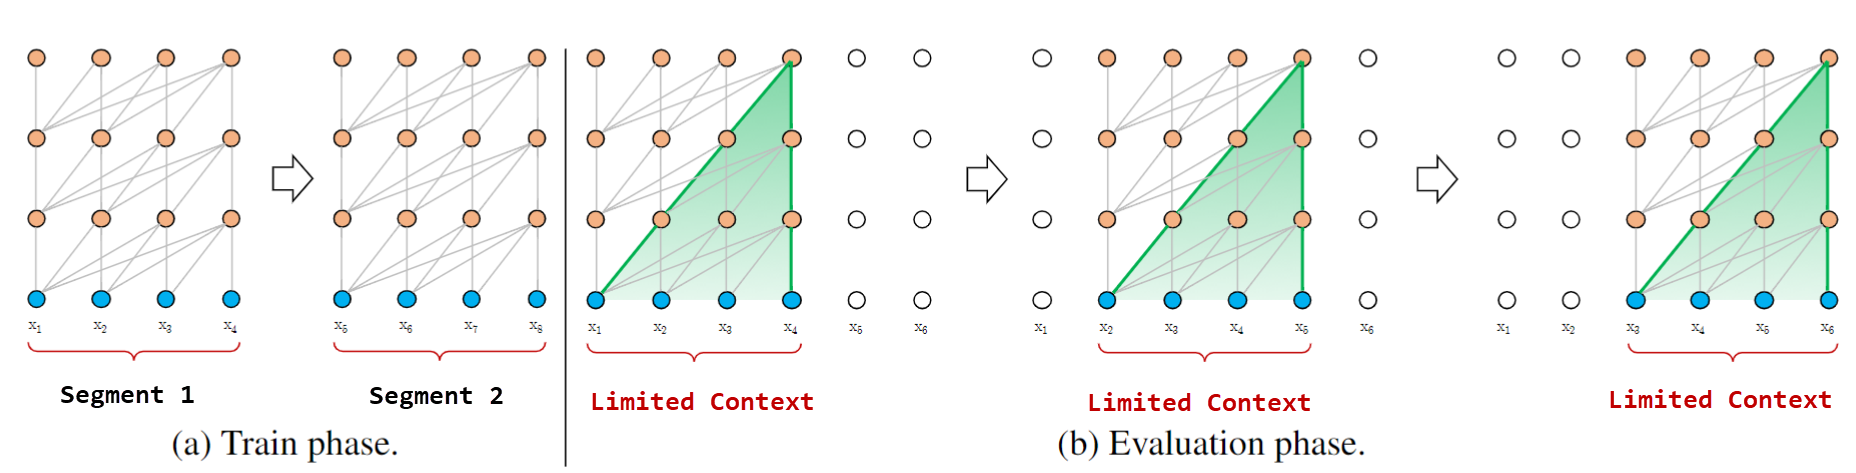
\includegraphics[width=0.99\textwidth]{imgs/transXL_vanillaSegmentation.png}
    %\vspace{-5pt}
    \caption{\small Vanilla Transformer with segment embedding length $ = 4$. Training the model in fixed-length segments while disregarding natural sentence boundaries results in the \emph{context fragmentation problem}: during each evaluation step, the Transformer consumes a segment embedding and makes a prediction at the last position. Then {\color{Teal} at the next step, the segment is shifted right by one position only, and the new segment must be processed from scratch, so there is no context dependency for first tokens of each segment and between segments.} From \emph{Transformer-XL: Attentive Language Models Beyond a Fixed-Length Context}, by Dai et al., 2019. \url{https://arxiv.org/pdf/1901.02860.pdf}. Copyright 2019 by Dai et al.}
    \vspace{-5pt}
    \label{fig:transXL_VanillaSegment}
    \end{figure}
    
\end{frame}



\begin{frame}{Motivation for Transformer-XL}

    \large 
    \linespread{0.5}
    
    \begin{itemizeSpaced}{15pt}
        \item \textbf{Transformer-XL} (extra long) learns longer dependencies without ``disrupting temporal coherence"  (Dai et al., 2019). 
        
        \item Doesn't chop sentences into arbitrary \textbf{fixed lengths}!
        
        \pinkbox Transformer-XL \emph{respects natural language boundaries} like sentences and paragraphs, helping it gain richer context over sentences, paragraphs, and even longer texts like documents. 
        
        \pinkbox Transformer-XL is composed of \textbf{segment-level recurrence mechanism} and \textbf{relative positional encoding} method (to fix \textbf{context fragmentation} and represent longer-spanning dependencies)
    \end{itemizeSpaced}
    
\end{frame}


\begin{frame}{Transformer-XL: Segment-Level Recurrence Mechanism}

    \linespread{0.3}
    
    When a segment is being processed, each hidden layer receives two inputs: 
    
    \begin{itemizeSpaced}{10pt}
        \item the previous hidden layer outputs of the \emph{current segment} (like vanilla transformer, visible as gray arrows in \cref{fig:transXL_extendedContext})
        
        \item the previous hidden layer outputs of the \emph{previous segment} (green arrows in \cref{fig:transXL_extendedContext}).
    \end{itemizeSpaced}
    
    
    
    \begin{figure}[h]
    \vspace{-5pt}
    \centering
    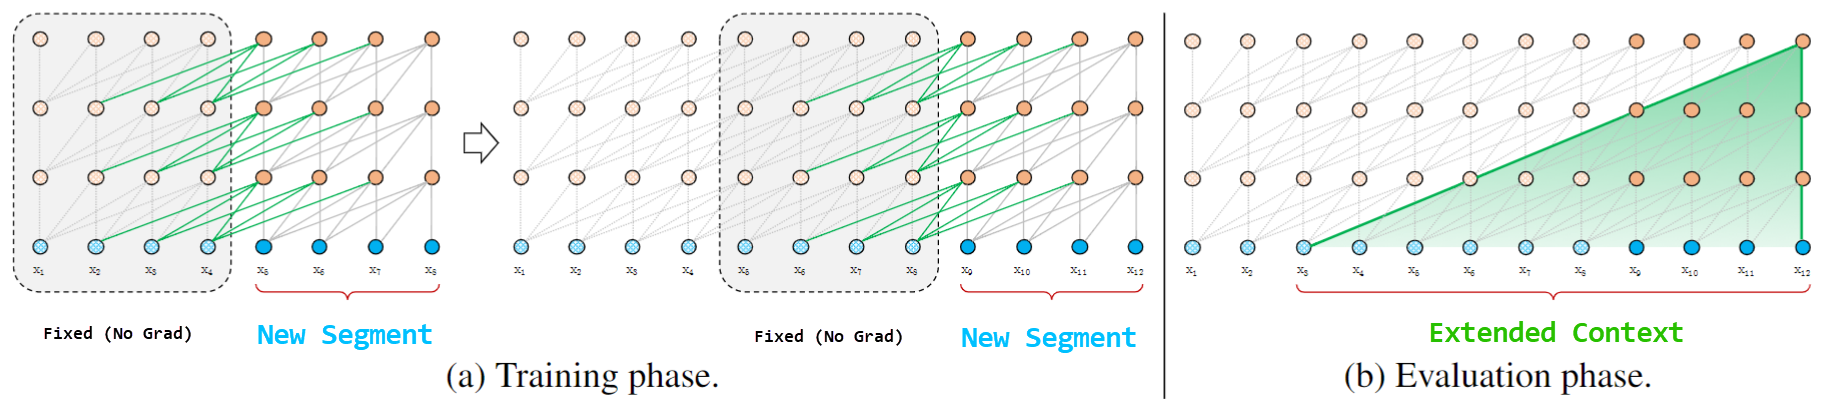
\includegraphics[width=0.99\textwidth]{imgs/transXL_extendedcontext.png}
    %\vspace{-5pt}
    \caption{\small Segment level recurrence mechanism at work: the hidden state for previous segment is \emph{fixed} and \emph{stored} to later be reused as extended context while new segment is processed. Like in Transformer, gradient updates (training) still occurs within a segment, but extended context includes historical information. From \emph{Transformer-XL: Attentive Language Models Beyond a Fixed-Length Context}, by Dai et al., 2019. \url{https://arxiv.org/pdf/1901.02860.pdf}. Copyright 2019 by Dai et al.}
    %\vspace{-5pt}
    \label{fig:transXL_extendedContext}
    \end{figure}
    
\end{frame}



\begin{frame}{Transformer-XL: Relative Positional Encoding}
    \normalsize\linespread{1.0}

    \begin{alertBlock}{Problem when using Segment-Level Recurrence}
    
        How can positional word order be kept coherent when reusing hidden states?
        
        Standard Transformer uses positional encodings (use absolute distance between tokens) .
    
        \begin{addmargin}{3em}{} % 3em left, NOTHING right
        \begin{itemizeSpaced}{5pt}
            \largearrowitem Applying to Transformer-XL caused consecutive word embedding sequences to be associated with the same positional encoding.
            
            \largearrowitem Tokens from different segments had the same positional encodings
            
            \largearrowitem Transformer-XL couldn't distinguish the difference in positions of consecutive input tokens.
            
            \largearrowitem Defeated the purpose of positional encodings!
            
        \end{itemizeSpaced}
        \end{addmargin} 
        
        
    \end{alertBlock} 
    
    {\large \textbf{Solution: Relative Positional Encodings}}
    
    \begin{itemizeSpaced}{0pt}
        \item uses \emph{relative} distance between tokens 
        
        \item injects this into \emph{each} attention score of each layer (rather than before first layer).
    \end{itemizeSpaced}

    
\end{frame}



\begin{frame}{Transformer-XL: Experimental Results}
    
    Ablation study: Isolating effects of \textbf{segment-level recurrence mechanism} with different encoding schemes (Shaw (2018) uses relative, and Vaswani / Al-Rfou use absolute).
        
    \begin{itemize}
        \item \textbf{KEY: }best results obtained using \emph{both}  segment-level recurrence and relative positional encoding.
    \end{itemize}
        
    
    \begin{figure}[h]
    \vspace{-5pt}
    \centering
    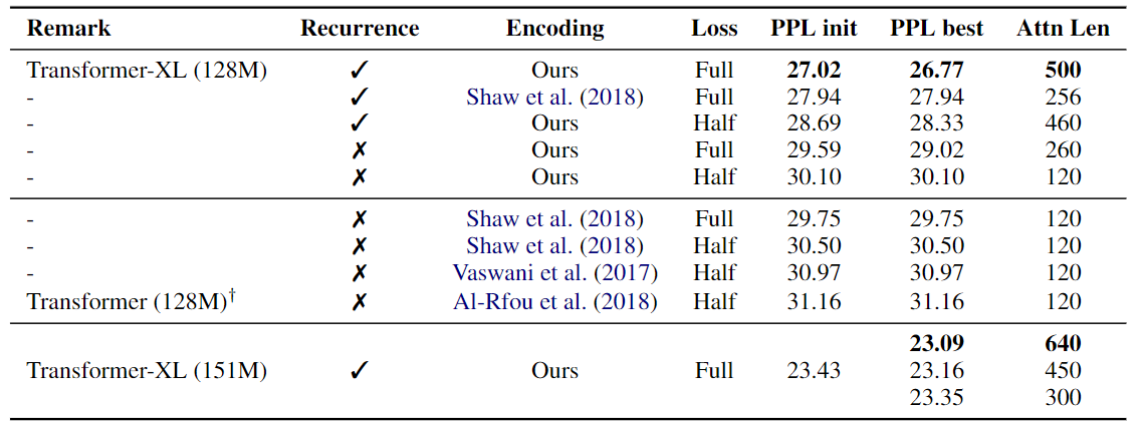
\includegraphics[width=0.99\textwidth]{imgs/table_transXL_ablationREC.png}
    \vspace{-5pt}
    \captionof{table}{\linespread{0.3}\footnotesize Ablation study for segment-level recurrence on the WikiText-103 data set. \textbf{PPL best} (model output) means perplexity score obtained using an optimal backpropagation training time length. \textbf{Attn Len} (model input) is the shortest possible attention length during evaluation to achieve the corresponding PPL best. From \emph{Transformer-XL: Attentive Language Models Beyond a Fixed-Length Context}, by Dai et al., 2019. \url{https://arxiv.org/pdf/1901.02860.pdf}. Copyright 2019 by Dai et al.}
    \vspace{-5pt}
    \label{tbl:transXL_ablationRECURR}
    \end{figure}

\end{frame}